\section{Organisation du projet}

\subsection{Les outils utilisés}


\subsection{Le planning initial}

Afin d'achever au mieux les objectifs que nous nous étions fixés, nous avons dressé un planning optimal des tâches à effectuer, en les répartissant par priorité. Voici le gantt des objectifs initiaux.

\begin{figure}[!ht]
    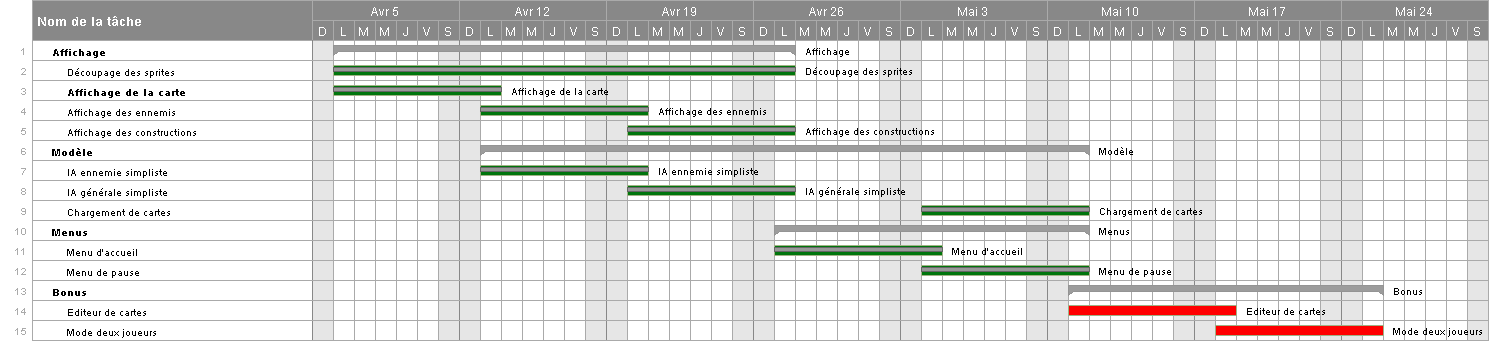
\includegraphics[width=1.1\textwidth]{./images/gantt.png}
    \caption{Gantt du projet}
\end{figure}

\subsection{UML des fichiers et fonctionnalités}

Voici le schéma simplifié de la structure des fichiers. Seuls les structures et fonctions les plus importantes ont été représentées afin de conserver la lisibilité du schéma. 

\begin{figure}[!ht]
    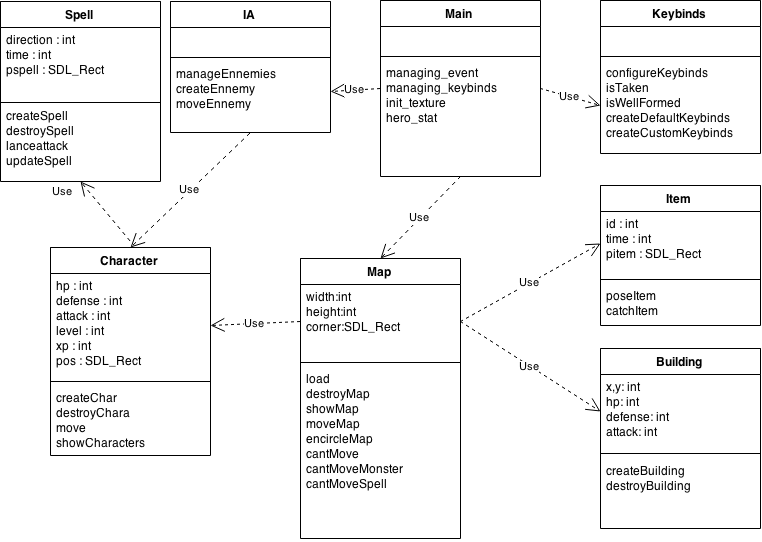
\includegraphics[width=1\textwidth]{./images/uml.png}
    \caption{UML}
\end{figure}

On peut remarquer l'organisation structurelle du code qui tend à se rapprocher d'un code objet. Les listes chaînées n'ont pas été représentées afin de ne pas encombrer l'UML.

